\section{End-to-End Object Detection with Transformers (DETR)}

\label{appendix:detr-paper}

\subsection{Overview}

\par Carion \textit{et al} in their 2020 paper titled \textit{End-to-End Object Detection with Transformers} aims to streamline the detection pipeline by effectively removing the need for many hand-designed components by introducing a DEtection TRansformer or DETR which includes set-based global loss that forces unique predictions via bipartite matching, and a transformer encoder-decoder architecture \cite{carion2020detr}.

\subsection{DETR Model}
\par Paper proposed two essential components for direct set predictions in detection: \par
\begin{itemize}
	\item Set prediction loss forces unique matching between ground truth boxes and predicted boxes.
	\item An architecture that predicts a set of objects and models their relation in a single pass.
\end{itemize}

\subsubsection{Object detection set prediction loss}
\begin{itemize}
	\item loss finds the optimal bipartite match between predicted and ground truth objects and then optimises object-specific (bounding box) losses. 
	\item We pad the ground truth object with no objects if there are fewer objects in it to achieve one-to-one matching for direct set prediction without duplicates.
	$$\hat{\sigma} = \arg \max_{\sigma \in \mathfrak{S}_N} \displaystyle\sum\limits_{i}^N L_{match}(yi, \hat{y}_{\sigma(i)})$$
	
	\item The next step is to calculate the Hungarian loss function for all pairings that were matched in the previous stage.
	$$L_{Hungarian}(y, \hat{y}) = \displaystyle\sum\limits_{i=0}^N [-log\hat{p}_{\hat{\sigma} (i)}(c_i)\:+\:\mathbb{1}_{c_i\neq\phi}L_{box}(b_i, \hat{b}_{\hat{\sigma}}(i))]$$
\end{itemize}

\subsubsection{DETR architecture}
\begin{figure}[h]
	\centering
	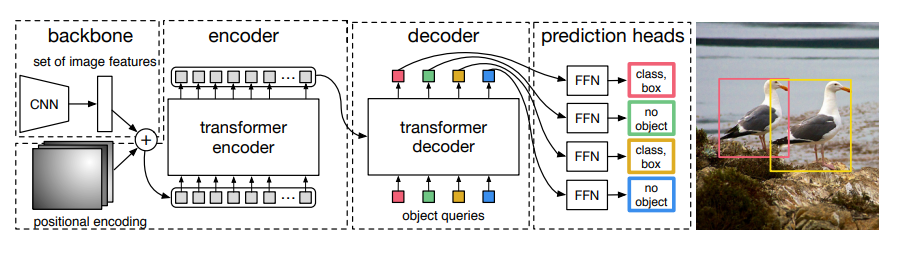
\includegraphics[width=\linewidth]{assets/img/detr-architecture.png}
	\caption{DETR architecture by Carion
		\textit{et al} (Courtesy \cite{carion2020detr})}
\end{figure}
\paragraph{Backbone}

\begin{itemize}
	\item It is a conventional CNN backbone which takes images as input and generates a lower-resolution activation map.
\end{itemize}	

\paragraph{Transformer encoder}

\begin{itemize}
	\item As the encoder expects a sequence as input, spatial dimensions are collapsed into one dimension, resulting in a d×HW feature map.
	\item Each encoder layer has a standard architecture that includes a multi-head self-attention module and a feed forward network (FFN).
	\item Since the transformer architecture is permutation-invariant, we supplement it with fixed positional encodings that are added to the input of each attention layer. 
\end{itemize}	

\paragraph{Transformer decoder}

\begin{itemize}
	\item The decoder follows the transformer's standard architecture, transforming N embeddings of size d with multi-headed self and encoder-decoder attention mechanisms.
	\item At each decoder layer, it decodes the N items in parallel. The N input embeddings must be distinct to produce different results because the decoder is permutation-invariant. These input embeddings are called object queries since they are learned positional encodings.
	\item The decoder converts the N object queries into an output embedding. A feed forward network decodes them independently into box coordinates and class labels, yielding N final predictions. 
\end{itemize}	

\paragraph{Prediction feed-forward networks}

\begin{itemize}
	\item The final prediction is computed by a 3-layer perceptron with ReLU activation function and hidden dimension d, and a linear projection layer. 
	\item It predicts the box's normalised centre coordinates, height, and width in relation to the input image, whereas the linear layer uses a softmax function to predict the class label. 
\end{itemize}	

\subsection{Conclusion}
\par Carion \textit{et al} present DETR \cite{carion2020detr}, a new design for object detection systems based on transformers and bipartite matching loss for direct set prediction. On the challenging COCO dataset, the technique produces results that are comparable to an optimised Faster R-CNN baseline. DETR is easy to set up and maintain, with a modular design that allows for easy expansion and competitive outcomes. Furthermore, it outperforms Faster R-CNN on huge objects.